\documentclass[11pt]{report}
% define the title
\usepackage[brazil]{babel}
\usepackage[utf8]{inputenc}		%Usar acentos diretos do teclado
\usepackage[T1]{fontenc}		%Padrão para imagens
\usepackage{graphicx}
\usepackage{subfigure}
\usepackage{rotating}
\usepackage{longtable}
\usepackage{amsmath}
\usepackage{amsfonts}
\usepackage{amssymb}
\usepackage{geometry}
\usepackage{caption}
\geometry{left=3cm, right=2cm, top=2cm, bottom=2cm}
% Title Page
\title{Draft}
\author{Pedro}

\begin{document}
\chapter{Considerações Adicionais sobre Adaptação de Segundo Nível}
\section{Projeção dos pesos alfa da adaptação de segundo nível numa área de incerteza dos parâmetros com fronteira convexa e suave.}

Seja:

\begin{equation}
\hat{\theta}_p = \bar{\Theta}\alpha 
\end{equation}

o modelo virtual criado a partir de uma combinação convexa de n+1 modelos de identificação. Tal que $\bar{\Theta}\in R^{(n+1)xn}$ e $\alpha \in R^{n+1}$ e $\hat{\theta}_p \in R^n$

Se $g(\theta)$ delimita uma região suave e convexa dentro da qual estão contidos os parâmetros da planta então a escolha dos parâmetros iniciais dos modelos de identificação (vértices do fecho convexo inicial) na adaptação de segundo nível implica no seguinte problema:\\

Como utilizar toda a informação disponível sobre a região de incerteza $g(\theta)$? Em outras palavras, como escolher os parâmetros dos modelos de identificação iniciais de forma que o fecho convexo no espaço de parâmetros englobe a fronteira $g(\theta)$ com o melhor ajuste possível?\\

Um fecho convexo delimitado por um número finito de vértices não tem uma fronteira suave e portanto é possível apenas minimizar o volume de fecho convexo "desperdiçado" com a escolha dos vértices. Desta forma nos propomos a criar uma lei de projeção para o vetor $\alpha$ de forma que, na fronteira de $g(\theta)$, $\alpha$ se mantenha na região de incerteza conhecida.\\

Assim temos um problema de projeção dos parâmetros $\alpha$ da adaptação de segundo nível onde seguimos os argumentos padrão para a projeção: $\dot{\alpha}$ permanece inalterado quando $\alpha$ se encontra no interior da região delimitada pelo conjunto $\Phi$ ou na fronteira com tendência a entrar e é projetado quando $\alpha$ se encontra na fronteira com tendência a sair.

\begin{figure}[!htpb]
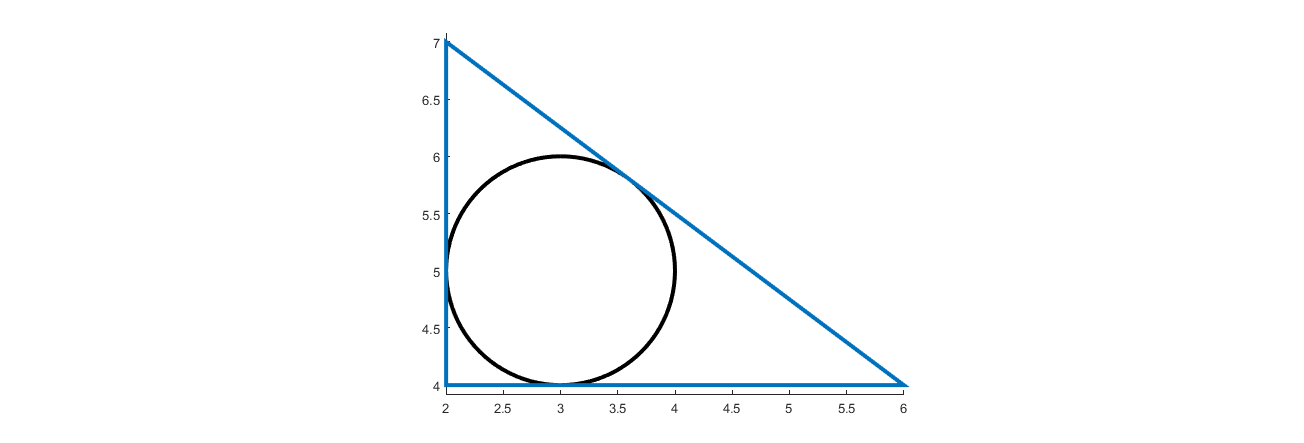
\includegraphics[width = \linewidth]{./pics/ilust.png}
\caption{Ilustração do problema, em preto uma fronteira suave e convexa $g(\theta)$ e em azul um fecho convexo delimitado por 3 vértices no $R^2$. A escolha dos mesmos no problema da adaptação de segundo nível implica que a estimativa $\hat{\theta}_p$ criada a partir da combinação convexa pode ter sua trajetória passando por fora da região de incerteza}

\end{figure}

Definimos uma região elipsóide em relação ao vetor $\theta$, centrada no ponto $\theta_c$:

\begin{equation}
g(\theta) = (\theta-\theta_c)^TP(\theta-\theta_c) - M^2
\end{equation}

onde $\theta\in R^n$, $\theta_c\in R^n$, $P=P^T \in R^{nxn}$ e $M$ é um escalar. O interior do elipsóide é caracterizado por $g(\theta)<0$ e sua fronteira por $g(\theta) = 0$. Denotamos o interior do elipsóide pela região $S$ e sua fronteira por $\delta(S)$.

Fazendo uma mudança de coordenadas para $\alpha$, obtemos diretamente outro elipsóide:

\begin{equation}
g(\alpha) = (\bar{\Theta}\alpha - \theta_c)^TP(\bar{\Theta}\alpha - \theta_c)
\end{equation}

o gradiente deste elipsóide é dado por:

\begin{equation}
\nabla g(\alpha) = 2\bar{\Theta}^TP\bar{\Theta}\alpha - 2\bar{\Theta}^TP\theta_c
\end{equation}

Seja a lei adaptativa para o modelo virtual usada na adaptação de segundo nível:

\begin{equation}
\dot{\bar{\alpha}} = -E^T(t)E(t)\alpha - E^T(t)e_{n+1}(t)
\end{equation}

Usando as definições anteriores estabelecemos a seguinte lei com projeção


\begin{equation}
\label{eq:sigmaIDMARC}
\displaystyle \dot{{\alpha}} = \left\{
\begin{array}{rl}
        \dot{\bar{\alpha}},          &\mbox{ se $\alpha \in S$ ou ($\alpha \in \delta(S)$ e}\\                         &\mbox{$\dot{\bar{\alpha}}^T\nabla g(\alpha) < 0 $} \\
        \Pr(\dot{\bar{\alpha}}), &\mbox{caso contrário}
\end{array} \right.
\end{equation}

Onde $Pr(\dot{\bar{\alpha}})$ é obtido extraindo a componente do vetor na mesma direção do gradiente:

\begin{equation}
Pr(\dot{\bar{\alpha}}) = \dot{\bar{\alpha}} - \nabla g^T \dot{\bar{\alpha}} \nabla g (\nabla g^T \nabla g)^{-1}
\end{equation}

Finalmente, temos o problema descrito no apêndice B do livro do Ioannou, onde é possível, com essa lei de projeção para um elipsóide, que o vetor resultante da iteração seguinte na simulação esteja fora da região de incerteza definida pelo elipsóide. Desta forma, fazemos o seguinte raciocínio: Se um vetor se encontra próximo à fronteira de um dado elipsóide, trazer o vetor até a fronteira é apenas uma questão de andar na direção apropriada do gradiente: 
\begin{equation}
\alpha_{k+1}^{ajustado} = \alpha_{k+1} - L\nabla g
\end{equation}


desta forma resolvemos a seguinte equação de segundo grau no escalar $L$, caso $g(\alpha_{k+1})>0$.

\begin{equation}
(\bar{\Theta}(\alpha - L\nabla g) - \theta_c)^TP(\bar{\Theta}(\alpha - L\nabla g) - \theta_c) - M^2 = 0
\end{equation}

de onde obtemos os coeficientes $a,b,c$ da equação de segundo grau em $L$\\
$aL^2 +bL + c = 0$, onde:

\begin{equation}
a = \nabla g^T \bar{\Theta} P \bar{\Theta} \nabla g
\end{equation}

e
 
\begin{equation}
b = -\alpha^T \bar{\Theta}^T P \bar{\Theta} \nabla g - \nabla g^T\bar{\Theta}^TP\bar{\Theta}\alpha + \nabla g^T \bar{\Theta}^T P \theta_c + \theta_c^TP\bar{\Theta}\nabla g
\end{equation}

e finalmente:

\begin{equation}
c = \alpha^T \bar{\Theta}^T P \bar{\Theta \alpha} - \alpha^T \bar{\Theta}^TP\theta_c - \theta_c^TP\theta_c - M^2
\end{equation}

tal que:

\begin{equation}
L_{1,2} = (-b \pm \sqrt{b^2 - 4ac})/2a
\end{equation}

e $L = min(L_1, L_2)$\\

Aplicando esta lei de projeção, garantimos que $\alpha$ pertence à região de incerteza definida pelo elipsóide em $g(\alpha)$. Partindo deste argumento para uma única região, é possível expandir o raciocínio para a união de múltiplos elipsóides definidos por uma série de funções $g_i(\theta)$, de forma que é possível "desenhar" uma quantidade maior de regiões de incerteza de parâmetros.  

\section{Aprendizado Concorrente/Paralelo}

Em [CHOWDHARY,2010], foi introduzido o conceito de "concurrent learning" para o controle adaptativo convencional, onde a necessidade de um sinal com a característica de persistência de excitação (como por exemplo um sinal rico em frequências) para garantir a convergência das estimativas dos parâmetros da planta para seus valores corretos é removida, sendo no lugar necessário apenas que os dados usados para gerar a taxa de adaptação dos parâmetros sejam armazenados em um certo número de instantes distintos e que tais dados formem um conjunto linearmente independente.

No caso do controle adaptativo com adaptação de segundo nível, seja a equação de adaptação dos parâmetros $\alpha$ da seguinte forma (apresentada na forma original sem projeção):

\begin{equation}
\dot{\alpha} = -E^T(t)E(t)\alpha(t) - E^T(t)e_{n+1}(t)
\end{equation}

Notamos o seguinte fato: A dimensionalidade dos pontos de equilíbrio na equação está diretamente relacionada com o posto da matriz $E^T(t)E(t)$. De fato, quando existe excitação de magnitude suficiente em todos os modos da planta e dos modelos de identificação, o posto da matriz é cheio e está distante de uma matriz de posto deficiente. Desta forma existe apenas um único $\alpha$ tal que $\dot{\alpha}=0$. Caso sejamos capazes de armazenar os dados em diferentes instantes de tempo garantindo que matriz $M = \sum E_j^TE_j$ tem posto cheio, propomos a seguinte equação:

\begin{equation}
\dot{\alpha} = -E^T(t)E(t)\alpha(t) - E^T(t)e_{n+1}(t) -\sum E_j^TE_j\alpha(t) -\sum E_j^Te_{n+1,j}
\end{equation}

Seja a candidata à função de Lyapunov:

\begin{equation}
V(\tilde{\alpha}) = \frac{1}{2}\tilde{\alpha}^T\tilde{\alpha} 
\end{equation}

Seja $\alpha$ invariante, $\dot{\tilde{\alpha}} = \dot{\alpha}$, diferenciando obtemos:

\begin{equation}
\dot{V}(\tilde{\alpha}) = \tilde{\alpha}^T(-E^T(t)E(t)\alpha(t) - E^T(t)e_{n+1}(t) -\sum E_j^TE_j\alpha(t) -\sum E_j^Te_{n+1,j})
\end{equation}

Como $\tilde{\alpha} = \alpha - \alpha^*$, substituímos $\alpha = \tilde{\alpha} + \alpha^*$. Já que assumimos que existe uma única solução para $\alpha=\alpha^*$ tal que $\sum E^T_jE_j \alpha = -\sum E^T_je(n+1),j$ pois o posto da matriz $M$ é cheio e $\alpha^*$ também é uma solução de $\alpha$ para o instante presente mesmo que $E^T(t)E(t)$ não tenha posto cheio, podemos escrever $E^T(t)E(t)\alpha^* = -E^T(t)e_{n+1}(t)$, desta forma, substituindo:

\begin{equation}
\dot{V}(\tilde{\alpha}) = -\tilde{\alpha}(E^T(t)E(t)+\sum E_j^TE_j)(\tilde{\alpha}+\alpha^*) - \tilde{\alpha}(E^T(t)e_{n+1}(t) + \sum E_j^Te_{n+1},j)
\end{equation}

Mas $(E^T(t)E(t)+\sum E_j^TE_j)\alpha^* = -(E^T(t)e_{n+1}(t) + \sum E_j^Te_{n+1},j)$, desta forma obtemos cancelamento dos termos de sinal indefinido, obtendo:

\begin{equation}
\dot{V}(\tilde{\alpha}) = -\tilde{\alpha}(E^T(t)E(t)+\sum E_j^TE_j)\tilde{\alpha}
\end{equation}

Como para uma matriz qualquer temos sempre que $P^TP$ possui autovalores positivos ou nulos, sabemos que $(E^T(t)E(t)+\sum E_j^TE_j)>0$, e portanto $\dot{V}(\tilde{\alpha})<0$ e o sistema de identificação converge exponencialmente para a origem $\tilde{\alpha} = 0$
 
\end{document}